\documentclass{article}
\usepackage{graphicx} % Required for inserting images
\usepackage{authblk} % Required for author affiliations
\usepackage{indentfirst} % Indent first paragraph of sections
\usepackage{amssymb} % For mathematical symbols
\usepackage{amsthm} % For theorem environments
\usepackage{amsmath} % For advanced math typesetting
\usepackage{hyperref}
\usepackage{enumitem}
\usepackage{pgfplots} % For plots
\usepackage{tikz} % For drawing shapes
\usepackage{circuitikz}
\usepackage{float} % For [H] float option
\pgfplotsset{compat=1.18} % Set compatibility level
\usetikzlibrary{decorations.pathreplacing}
\newtheorem{theorem}{Theorem}
\newtheorem{law}{Law}
\newtheorem{principle}{Principle}
\newtheorem{corollary}{Corollary}[theorem]
\newtheorem{lemma}[theorem]{Lemma}
\newtheorem{definition}{Definition}
\newtheorem{problem}{Problem}
\newtheorem{solution}{Solution}
\newtheorem*{example}{Example}
\newtheorem{remark}{Remark}
\newtheorem{proposition}{Proposition}
\reversemarginpar
\hypersetup{
    colorlinks=true,
}
\begin{document}

% ============================================================
%  Title page
% ============================================================
\title{PHYS 350: Honours Electricity and Magnetism}
\author{W.R.YCH.}
\date{August \(31^{st}\), 2026}
\setcounter{Maxaffil}{0}
\renewcommand\Affilfont{\itshape\small}
\maketitle

% ============================================================
%  Abstract
% ============================================================
\noindent\rule{\textwidth}{0.4pt}
\thispagestyle{empty}
\begin{abstract}
\end{abstract}
\noindent\rule{\textwidth}{0.4pt}
\clearpage

% ============================================================
%  Table of Contents
% ============================================================
\thispagestyle{empty}
{
  \hypersetup{linkcolor=black}
  \tableofcontents
}
\clearpage

% ============================================================
\setcounter{page}{1}

% ============================================================
%  INTRODUCTION
% ============================================================
\section{Introduction}
Textbook used is David J. Griffiths - Introduction to Electrodynamics Fifth Edition. Course grading is divided as follows:
\begin{itemize}
    \item 35\% problem sets (must be handwritten scans).
    \item 25\% midterm.
    \item 40\% final exam.
\end{itemize}

\section{Vector Analysis}
\subsection{Terminologies}
\marginpar{August 31, 2026}
\begin{definition}[Scalar]
    A scalar is a quantity with just a magnitude.
\end{definition}
\begin{definition}[Vector]
    A vector is a quantity with a magnitude and a direction, i.e. $\vec{v} = v_x\hat{x} + v_y\hat{y} + v_z\hat{z}$.
\end{definition}
\begin{definition}[Cross Product]
    The cross product is a vector perpendicular to both, set by the right hand rule, and it vanishes for parallel vectors:
    \[\vec{v}\times\vec{w} = |\vec{v}||\vec{w}|\sin\theta\,\hat{n}
    = \begin{vmatrix} \hat{x} & \hat{y} & \hat{z} \\ v_x & v_y & v_z \\ w_x & w_y & w_z \end{vmatrix}
    = \hat{x}(v_yw_z - w_yv_z) - \hat{y}(v_xw_z - w_xv_z) + \hat{z}(v_xw_y - w_xv_y).\]
\end{definition}
\begin{definition}[Dot Product]
    The dot product measures how much of $\vec{v}$ points along $\vec{w}$, so it is zero for perpendicular vectors:
    \[\vec{v}\cdot\vec{w} = v_xw_x + v_yw_y + v_zw_z = |\vec{v}||\vec{w}|\cos\theta.\]
\end{definition}
\begin{remark}
    Note $\vec{v}\times\vec{w} = -\vec{w}\times\vec{v}$, and $|\vec{v}| = \sqrt{\vec{v}\cdot\vec{v}}$.
\end{remark}
\begin{definition}[Field]
    A field is something with a value at every point in space. A scalar field assigns a number to each point, like temperature $T(x,y,z)$ or the height of a hill. A vector field assigns a vector to each point, like fluid velocity or $\vec{E}$.
\end{definition}

\subsection{Differential Calculus}
\marginpar{September 2, 2026}
\begin{definition}[Del operator]
    The del operator
    \[\vec{\nabla} = \left(\frac{\partial}{\partial x}, \frac{\partial}{\partial y}, \frac{\partial}{\partial z}\right).\]
\end{definition}
\begin{definition}[Gradient]
    The gradient turns a scalar into a vector, pointing in the direction of steepest increase of $f$:
    \[\vec{\nabla}f = \frac{\partial f}{\partial x}\hat{x} + \frac{\partial f}{\partial y}\hat{y} + \frac{\partial f}{\partial z}\hat{z}.\]
\end{definition}
\begin{remark}
    The gradient points in the steepest uphill direction, and its length grows where the hill is steeper. It is always perpendicular to the contours of constant $f$.
\end{remark}
\begin{definition}[Divergence]
    Divergence turns a vector into a scalar, measuring sources and sinks. For a small box, non-zero divergence means the inflow and outflow through its faces do not balance: arrows spreading from a point (positive) mean fluid is created there, arrows converging (negative) mean it is destroyed.
    \[\vec{\nabla}\cdot\vec{F} = \frac{\partial F_x}{\partial x} + \frac{\partial F_y}{\partial y} + \frac{\partial F_z}{\partial z}.\]
\end{definition}
\begin{definition}[Curl]
    Curl turns a vector into a vector, measuring local rotation. Picture a small paddle wheel: if the flow spins it, the curl is non-zero there. Uniform flow does not spin it, but shear flow (parallel arrows, longer on one side) does, so straight field lines do not imply zero curl.
    \[\vec{\nabla}\times\vec{F} = \begin{vmatrix} \hat{x} & \hat{y} & \hat{z} \\[2pt] \frac{\partial}{\partial x} & \frac{\partial}{\partial y} & \frac{\partial}{\partial z} \\[2pt] F_x & F_y & F_z \end{vmatrix}.\]
\end{definition}


\subsection{Integral Calculus}
\begin{definition}[Integral]
    An integral is an instruction to move along a region, evaluate something at each step, and add it to a running total.
\end{definition}
\begin{definition}[Line Integral]
    A line integral sums $\vec{F}$ along a curve, picking up only the component tangent to the path:
    \[\int_C \vec{F}\cdot d\vec{l}.\]
\end{definition}
\begin{example}
    Take $\vec{F} = y\hat{x}$ along a counterclockwise quarter circle of radius $R$. On the circle $d\vec{l} = R\,d\phi(-\sin\phi\,\hat{x} + \cos\phi\,\hat{y})$ and $y = R\sin\phi$, so
    \[\int_C \vec{F}\cdot d\vec{l} = -R^2\int_0^{\pi/2}\sin^2\phi\,d\phi = -\frac{R^2\pi}{4}.\]
    It is negative because $\vec{F}$ points along $+\hat{x}$ while we travel in the $-\hat{x}$ direction over most of the arc.
\end{example}
\begin{definition}[Flux]
    Flux measures how much of the field pokes through a surface:
    \[\int_S \vec{F}\cdot d\vec{a} = \int_S \vec{F}\cdot\hat{n}\,da.\]
\end{definition}
\begin{definition}[Volume Integral]
    A volume integral sums a scalar over a region, giving the mass if $f$ is a density:
    \[\int_V f\,d^3\vec{r} = \int_V f\,dx\,dy\,dz.\]
\end{definition}
\begin{remark}
    We write $\oint$ when the curve is a closed loop or the surface is closed.
\end{remark}

\subsubsection{The Three Fundamental Theorems}
Integrating a derivative over a region reduces to evaluating the original object on the boundary of that region.
\begin{theorem}[Gradient theorem]
    The boundary of a curve is two points:
    \[\int_a^b \vec{\nabla}h\cdot d\vec{l} = h(b) - h(a).\]
    To find my altitude change climbing a hill, I can compare before and after, or add up all the little changes along the way.
\end{theorem}
\begin{theorem}[Stokes' theorem]
    The boundary of a surface is a curve:
    \[\int_S (\vec{\nabla}\times\vec{F})\cdot d\vec{a} = \oint_C \vec{F}\cdot d\vec{l}.\]
    To get the total swirl, I can work out the rotation at the boundary, or add up all the little whirlpools inside. Neighbouring whirlpools cancel along their shared edges, leaving only the boundary.
\end{theorem}
\begin{theorem}[Gauss' divergence theorem]
    \label{Gauss-div}
    The boundary of a volume is a surface:
    \[\int_V (\vec{\nabla}\cdot\vec{F})\,d^3\vec{r} = \oint_S \vec{F}\cdot d\vec{a}.\]
    To find the total flux leaking out through the surface, I can add up all the sources inside. Flux between neighbouring cells cancels, leaving only the outer surface.
\end{theorem}
\begin{definition}[Current density]
    The current $I$ through a wire is not a local quantity, since a wire has finite thickness. The local version is the current density
    \[\vec{J} = \frac{d\vec{I}}{da_\perp},\]
    where $da_\perp$ is the differential cross section perpendicular to the flow.
\end{definition}
\begin{remark}
    The divergence theorem \ref{Gauss-div} applied to $\vec{J}$ is how the conservation of charge gets written down.
\end{remark}

\subsection{Index Notation}
\marginpar{September 4, 2026}
\begin{remark}
    A matrix carries two indices, $A_{ij}$, where $i$ says which row and $j$ says which column.
\end{remark}
\begin{definition}[Transpose]
    The transpose swaps the indices, $(A^T)_{ij} = A_{ji}$.
\end{definition}
\begin{definition}[Symmetry]
    A symmetric matrix has $A_{ij} = A_{ji}$, and an antisymmetric one has $B_{ij} = -B_{ji}$.
\end{definition}
\begin{definition}[Kronecker delta]
    The Kronecker delta equals $+1$ when its condition is fulfilled and $0$ otherwise, so it could be the identity matrix in index notation:
    \[\delta_{ij} = \begin{cases} +1 & i = j \\ 0 & i \neq j \end{cases}.\]
\end{definition}
\begin{example}
    \[\sum_j \delta_{ij}v_j = v_i.\]
\end{example}
\begin{proposition}[Matrix Multiplication]
    \[\vec{w} = A\vec{v} \implies w_i = \sum_j A_{ij}v_j.\]
\end{proposition}
\begin{proposition}[Dot Product]
    \[\vec{v}\cdot\vec{w} = \sum_i v_iw_i.\]
\end{proposition}
\begin{proposition}[Cross Product]
    \[(\vec{v}\times\vec{w})_i = \sum_{j,k}\varepsilon_{ijk}v_jw_k.\]
\end{proposition}
\begin{definition}[Levi-Civita symbol]
    $\varepsilon_{ijk}$ is defined by
    \begin{itemize}
        \item $\varepsilon_{123} = +1$, and cyclic permutations keep the sign: $\varepsilon_{123} = \varepsilon_{231} = \varepsilon_{312}$.
        \item Swapping any two indices flips the sign, so $\varepsilon_{321} = \varepsilon_{213} = \varepsilon_{132} = -1$.
        \item If any two indices are equal, $\varepsilon_{ijk} = 0$.
    \end{itemize}
\end{definition}
\begin{example}
    For $i = 1$, only the terms with $(j,k) = (2,3)$ and $(3,2)$ survive:
    \[(\vec{v}\times\vec{w})_1 = \varepsilon_{123}v_2w_3 + \varepsilon_{132}v_3w_2 = v_2w_3 - v_3w_2.\]
\end{example}
\begin{proposition}[Epsilon-delta identity]
    Contracting two Levi-Civita symbols on a shared index gives
    \[\sum_i \varepsilon_{ijk}\varepsilon_{imn} = \delta_{jm}\delta_{kn} - \delta_{jn}\delta_{km}.\]
\end{proposition}

\subsection{Second Derivatives Identities}
\begin{definition}[Laplacian]
    Taking the divergence of a gradient gives
    \[\vec{\nabla}\cdot(\vec{\nabla}f) = \frac{\partial^2 f}{\partial x^2} + \frac{\partial^2 f}{\partial y^2} + \frac{\partial^2 f}{\partial z^2} \equiv \nabla^2 f,\]
    where $\nabla^2$ is the Laplacian\footnote{Mathematicians often write $\Delta$, but in physics we use $\nabla^2$.}.
\end{definition}
\begin{example}[Sign of the Laplacian]
    At a local maximum $\vec{\nabla}f$ points inward from every side, so it has negative divergence and $\nabla^2 f < 0$; at a minimum, $\nabla^2 f > 0$. At a saddle the second derivatives can cancel, so a flat point alone tells you nothing.
\end{example}
The full list of second derivative identities:
\begin{description}
    \item[Divergence of a gradient.] $\vec{\nabla}\cdot(\vec{\nabla}f) = \nabla^2 f$.
    \item[Curl of a gradient.] $\vec{\nabla}\times(\vec{\nabla}f) = 0$.
    \item[Divergence of a curl.] $\vec{\nabla}\cdot(\vec{\nabla}\times\vec{F}) = 0$.
    \item[Identity 1.] $\vec{\nabla}\times(\vec{\nabla}\times\vec{F}) = \vec{\nabla}(\vec{\nabla}\cdot\vec{F}) - \nabla^2\vec{F}$.
\end{description}

\subsubsection{Proving the Identities}
\subsubsection*{Curl of a Curl}
Set $\vec{G} \equiv \vec{\nabla}\times(\vec{\nabla}\times\vec{F})$. Then,
\[G_i = \sum_{j,k}\varepsilon_{ijk}\partial_j\sum_{m,n} \varepsilon_{kmn}\partial_m F_n=\sum_{j,k,m,n}\varepsilon_{ijk}\varepsilon_{kmn}\partial_j\partial_mF_n.\]
The shared index $k$ is in the third slot of the first symbol, so rotate it forward with the cyclic property $\varepsilon_{ijk} = \varepsilon_{kij}$ to match the proposition ($k$ now first in both):
\[\sum_k \varepsilon_{kij}\varepsilon_{kmn} = \delta_{im}\delta_{jn} - \delta_{in}\delta_{jm}.\]
Reading off the proposition with the summed index $k$ removed: the leftover pairs are $(i,j)$ and $(m,n)$, giving straight ($\delta_{im}\delta_{jn}$) minus crossed ($\delta_{in}\delta_{jm}$). Hence
\[G_i = \sum_{j,m,n}\left(\delta_{im}\delta_{jn} - \delta_{in}\delta_{jm}\right)\partial_j\partial_m F_n.\]
Each Kronecker delta collapses one sum by setting its indices equal. In the first term $\delta_{im}$ forces $m = i$ and $\delta_{jn}$ forces $n = j$; in the second, $\delta_{in}$ forces $n = i$ and $\delta_{jm}$ forces $m = j$:
\[G_i = \sum_j \partial_j\partial_i F_j - \sum_j \partial_j\partial_j F_i.\]
The first term is $\partial_i\sum_j\partial_j F_j = \left(\vec{\nabla}(\vec{\nabla}\cdot\vec{F})\right)_i$ and the second is $-(\nabla^2\vec{F})_i$, giving $\vec{\nabla}\times(\vec{\nabla}\times\vec{F}) = \vec{\nabla}(\vec{\nabla}\cdot\vec{F}) - \nabla^2\vec{F}$.

\subsubsection*{Curl of a Gradient}
Start from the definition, with $\vec{\nabla}f=\partial_k f$:
\[\left(\vec{\nabla}\times(\vec{\nabla}f)\right)_i = \sum_{j,k}\varepsilon_{ijk}\partial_j\partial_k f.\]
Call this sum $S$. Since $j$ and $k$ are both summed over, they are dummy labels and can be renamed freely; swap $j \leftrightarrow k$ everywhere:
\[S = \sum_{j,k}\varepsilon_{ikj}\partial_k\partial_j f.\]
Now clean up the two factors. Antisymmetry of $\varepsilon$ gives $\varepsilon_{ikj} = -\varepsilon_{ijk}$, and partial derivatives commute so $\partial_k\partial_j f = \partial_j\partial_k f$. Hence
\[S = -\sum_{j,k}\varepsilon_{ijk}\partial_j\partial_k f = -S.\]
So $S = -S$, which forces $S = 0$. Therefore $\vec{\nabla}\times(\vec{\nabla}f) = 0$.

\subsection{The Theory of Vector Fields}
\begin{definition}[Irrotational and solenoidal]
    A field with $\vec{\nabla}\times\vec{F} = 0$ everywhere is irrotational; a field with $\vec{\nabla}\cdot\vec{F} = 0$ everywhere is solenoidal.
\end{definition}
\begin{theorem}[Helmholtz]
    If $\vec{\nabla}\cdot\vec{F}$ and $\vec{\nabla}\times\vec{F}$ are specified everywhere and $\vec{F}\to 0$ at infinity, then $\vec{F}$ is uniquely determined. It can be written as $\vec{F} = \vec{\nabla}\psi + \vec{\nabla}\times\vec{A}$, an irrotational part plus a solenoidal part.
\end{theorem}
\begin{theorem}[Irrotational fields]
    Let $\vec{F}$ be a $C^1$ vector field on a simply connected domain (e.g.\ all of $\mathbb{R}^3$). The following are equivalent:
    \begin{enumerate}[label=(\roman*)]
        \item $\vec{\nabla}\times\vec{F} = 0$ everywhere.
        \item $\int_a^b \vec{F}\cdot d\vec{l}$ is independent of path, for any given end points.
        \item $\oint_C \vec{F}\cdot d\vec{l} = 0$ for every closed loop $C$.
        \item $\vec{F} = -\vec{\nabla}\psi$ for some scalar field $\psi$.
    \end{enumerate}
\end{theorem}
\begin{theorem}[Solenoidal fields]
    Let $\vec{F}$ be a $C^1$ vector field on a domain with no enclosed voids (e.g.\ all of $\mathbb{R}^3$). The following are equivalent:
    \begin{enumerate}[label=(\roman*)]
        \item $\vec{\nabla}\cdot\vec{F} = 0$ everywhere.
        \item $\int_S \vec{F}\cdot d\vec{a}$  is independent of surface, for any given boundary line.
        \item $\oint_S \vec{F}\cdot d\vec{a} = 0$ for any closed surface $S$.
        \item $\vec{F} = \vec{\nabla}\times\vec{A}$ for some vector field $\vec{A}$.
    \end{enumerate}
\end{theorem}

\section{Electrostatics}
\subsection{Electric Field}
\marginpar{September 11, 2026}
\begin{law}[Coulomb's law]
    The force on a point charge $q_2$ due to a point charge $q_1$ is
    \begin{equation}
        \vec{F} = \frac{1}{4\pi\epsilon_0}\frac{q_1q_2}{\mathfrak{r}^2}\,\hat{\mathfrak{r}},
    \end{equation}
    where $\vec{\mathfrak{r}}$ points from $q_1$ to $q_2$.\footnote{Coulomb's law has the same shape as Newton's gravity. The reason is geometric rather than a coincidence, and Gauss' law makes that explicit: in $d$ spatial dimensions the flux spreads over a $(d-1)$-dimensional sphere, so $F\propto 1/\mathfrak{r}^{d-1}$, and the $4\pi$ is the area of the unit sphere in $d=3$.}
\end{law}
\begin{definition}[Permittivity of free space]
    The permittivity of free space measures how easily an electric field can form in a classical vacuum:
    \[\epsilon_0 = 8.85 \times 10^{-12}\ \mathrm{C^2/(N\cdot m^2)}.\]
\end{definition}
\begin{definition}[Electric field]
    The electric field is the force per unit test charge. For a set of point charges $q_i$,
    \begin{equation}
        \vec{E}(\vec{r}) = \frac{1}{4\pi\epsilon_0}\sum_{i=1}^{n}\frac{q_i}{\mathfrak{r}_i^2}\,\hat{\mathfrak{r}}_i,
        \qquad \vec{\mathfrak{r}}_i \equiv \vec{r} - \vec{r}_i.
    \end{equation}
\end{definition}

\subsubsection{Continuous Charge Distributions}
\begin{definition}[Continuous distributions]
    Replacing $q_i$ by $dq = \lambda\,dl' = \sigma\,da' = \rho\,d\tau'$ turns the sum into an integral:
    \begin{equation}
        \vec{E}(\vec{r}) = \frac{1}{4\pi\epsilon_0}\int\frac{dq}{\mathfrak{r}^2}\,\hat{\mathfrak{r}},
        \qquad \vec{\mathfrak{r}} = \vec{r} - \vec{r}',
    \end{equation}
    where $\vec{r}$ is the field point and $\vec{r}'$ the source point.
\end{definition}

\marginpar{September 14, 2026}
\begin{example}[Finite line of charge]
    A line of length $2L$ along the $x$ axis carries uniform $\lambda$. Find $\vec{E}$ at $P = (0,0,z)$.
        \begin{figure}[H]
        \centering
        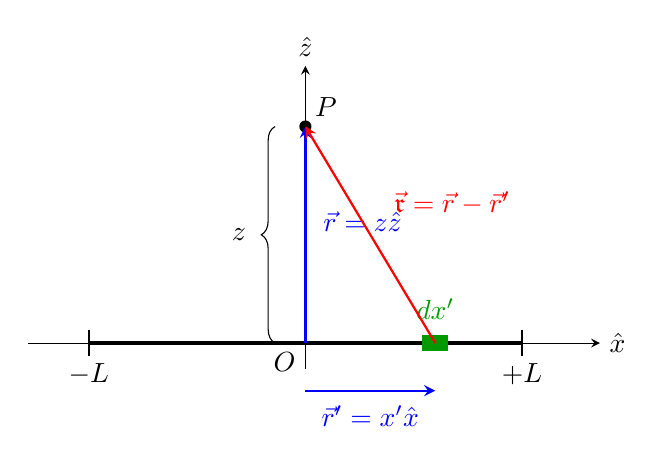
\begin{tikzpicture}[scale=1.1, >=stealth]
            % axes
            \draw[->] (-3.2,0) -- (3.4,0) node[right] {$\hat{x}$};
            \draw[->] (0,-0.3) -- (0,3.2) node[above] {$\hat{z}$};
            % line of charge
            \draw[line width=1.6pt] (-2.5,0) -- (2.5,0);
            \foreach \x in {-2.5,2.5} \draw[thick] (\x,0.15) -- (\x,-0.15);
            \node[below=4pt] at (-2.5,0) {$-L$};
            \node[below=4pt] at (2.5,0) {$+L$};
            \node[below left] at (0,0) {$O$};
            % element dx'
            \fill[green!60!black] (1.35,-0.09) rectangle (1.65,0.09);
            \node[above=2pt, green!60!black] at (1.5,0.1) {$dx'$};
            % field point
            \fill (0,2.5) circle (2pt) node[above right] {$P$};
            % r vector, label on the right
            \draw[->, thick, blue] (0,0) -- (0,2.5);
            \node[blue, right=3pt] at (0,1.4) {$\vec{r} = z\hat{z}$};
            % r' vector, drawn just below the axis
            \draw[->, thick, blue] (0,-0.55) -- (1.5,-0.55);
            \node[blue, below=2pt] at (0.75,-0.55) {$\vec{r}' = x'\hat{x}$};
            % separation vector
            \draw[->, thick, red] (1.5,0) -- (0,2.5);
            \node[red, above right=2pt] at (0.85,1.3) {$\vec{\mathfrak{r}} = \vec{r} - \vec{r}'$};
            % brace for z on the left
            \draw[decorate, decoration={brace, amplitude=5pt}] (-0.35,0) -- (-0.35,2.5)
                node[midway, left=7pt] {$z$};
        \end{tikzpicture}
        \caption{Setup for the finite line of charge. The source point $\vec{r}' = x'\hat{x}$ runs from $-L$ to $L$; the field point is $P$ at $\vec{r} = z\hat{z}$; the separation vector is $\vec{\mathfrak{r}} = \vec{r} - \vec{r}'$.}
    \end{figure}
    With $\vec{r} = z\hat{z}$ and $\vec{r}' = x'\hat{x}$,
    \[\vec{\mathfrak{r}} = z\hat{z} - x'\hat{x}, \qquad\mathfrak{r} = \sqrt{z^2 + x'^2},\]
    so
    \[\vec{E} = \frac{\lambda}{4\pi\epsilon_0}\int_{-L}^{L}\frac{z\hat{z} - x'\hat{x}}{(z^2 + x'^2)^{3/2}}\,dx'.\]
    The $\hat{x}$ term is odd in $x'$ and vanishes by symmetry. Using $\int dx'/(z^2 + x'^2)^{3/2} = x'/\big(z^2\sqrt{z^2 + x'^2}\big)$,
    \[\vec{E} = \frac{\lambda}{2\pi\epsilon_0 z}\cdot\frac{L}{\sqrt{L^2 + z^2}}\,\hat{z}.\]
    \begin{itemize}
        \item $z \ll L$: $\vec{E} \to \dfrac{\lambda}{2\pi\epsilon_0 z}\hat{z}$, the infinite line.
        \item $z \gg L$: $\vec{E} \to \dfrac{Q}{4\pi\epsilon_0 z^2}\hat{z}$ with $Q = 2\lambda L$, a point charge.
    \end{itemize}
\end{example}
\begin{remark}
    Always check limits: a finite distribution should reduce to a simpler known field up close and far away.
\end{remark}

\subsection{Gauss' Law}
\begin{law}[Gauss' law]
    The flux of $\vec{E}$ through any closed surface is set by the charge inside it:
    \begin{equation}
        \oint_S \vec{E}\cdot d\vec{a} = \frac{Q_{\text{enc}}}{\epsilon_0},
        \qquad Q_{\text{enc}} = \int_V \rho\,d\tau.
    \end{equation}
    Applying the divergence theorem to the left side gives $\int_V(\vec{\nabla}\cdot\vec{E})\,d\tau = \int_V (\rho/\epsilon_0)\,d\tau$. Since this holds for every volume $V$, the integrands match, giving the differential form
    \begin{equation}
        \vec{\nabla}\cdot\vec{E} = \frac{\rho}{\epsilon_0}.
    \end{equation}
\end{law}
\begin{remark}
    To solve for $\vec{E}$, choose a closed surface on which $E$ is constant and $\vec{E}$ is everywhere parallel or perpendicular to $d\vec{a}$, so $E$ comes out of the integral.
\end{remark}

\subsubsection{Spherical symmetry}
\begin{example}[Point charge]
    Surround a point charge $q$ with a sphere $S$ of radius $r$ centred on it. Two facts reduce the integral to a product:
    \begin{itemize}
        \item By symmetry, $\vec{E} = E(r)\,\hat{r}$: the field is radial and has the same magnitude everywhere on $S$.
        \item By geometry, $d\vec{a} = \hat{n}\,da = \hat{r}\,da$ on a sphere.
    \end{itemize}
    So $\vec{E}\cdot d\vec{a} = E\,da$, and
    \[
        \oint_S \vec{E}\cdot d\vec{a} = E\underbrace{\oint_S da}_{4\pi r^2} = \frac{q}{\epsilon_0}
        \quad\Longrightarrow\quad
        E = \frac{q}{4\pi\epsilon_0 r^2}.
    \]
    This is Coulomb's law, with $k = 1/4\pi\epsilon_0$.
\end{example}

\subsubsection{Cylindrical symmetry}
\begin{example}[Infinite line of charge]
    For a line with charge $\lambda$ per unit length, take a coaxial\footnote{Sharing a common central axis.} cylinder of radius $z$ and length $d$. $\vec{E}$ is radial, so the end caps carry no flux:
    \[E\,(2\pi z d) = \frac{\lambda d}{\epsilon_0}      \quad\Longrightarrow\quad E = \frac{\lambda}{2\pi\epsilon_0 z}.\]
    The field falls off as $1/z$, not $1/z^2$.
\end{example}

\begin{example}[Finite versus infinite line]
    Near the midpoint, a finite line gives a weaker field than an infinite one with the same $\lambda$. The same cylinder encloses the same charge, hence the same total flux, but for the finite line some of it leaks through the end caps, leaving less through the curved surface. The direct integration confirms this: the finite line field is the infinite line field times $L/\sqrt{L^2+z^2} < 1$.
\end{example}

\subsubsection{Why the fall-off depends on the geometry}
The exponent in the fall-off counts how much charge a cone of field lines can ``see'' as it grows. Picture a narrow cone opening from the observation point toward the source: its cross section at distance $r$ grows like $r^2$, which alone gives the $1/r^2$ dilution of a point charge. For extended sources, the charge inside the cone grows too:
\begin{itemize}
    \item Line of charge: the cone intercepts a length $\propto r$, so $E \propto r/r^2 = 1/r$.
    \item Sheet of charge: the cone intercepts an area $\propto r^2$, so $E \propto r^2/r^2$, a constant. The infinite sheet has a uniform field.
\end{itemize}
\begin{remark}
    For two equal positive charges, no field lines cross the midplane: the field there is parallel to the plane and vanishes at the midpoint. Gauss' law still holds, but without symmetry it cannot solve for $\vec{E}$.
\end{remark}

\marginpar{September 16, 2026}

\section{Potentials}
\section{Electric Fields in Matter}
\section{Magnetostatics}
\section{Magnetic Fields in Matter}
\section{Electrodynamics}

% ============================================================
%  APPENDIX
% ============================================================
\appendix
\section{Appendix}
\begin{remark}[Compactified dimensions]
    %Add this to the appendix useless info for exam
    Suppose an extra dimension exists but is curled up, the way a flat sheet with coordinates $(x,y)$ can be rolled into a cylinder whose second coordinate $w$ is periodic with a small radius. At distances much smaller than that radius, field lines spread out into all the dimensions and the field falls off faster than $1/r^2$. At distances much larger than it, there is only room to spread out in the large dimensions and the usual $1/r^2$ is recovered. So a measured deviation from the inverse square law at short range would be evidence for extra dimensions.

    This has been tested for gravity by the E\"ot-Wash torsion balance experiments (2004, 2007, 2020), which checked the $1/r^2$ law down to separations of $52\,\mu$m. Newtonian gravity fit the data, ruling out gravitational strength Yukawa interactions with ranges above $38.6\,\mu$m at 95\% confidence.
\end{remark}

% ============================================================
%  Useful Links
% ============================================================
\section{Useful Links}

\end{document}